%%%%%%%%%%%%%%%%%%%%%%%%%%%%%%%%%%%%%%%%%
% Arsclassica Article
% LaTeX Template
% Version 1.1 (1/8/17)
%
% This template has been downloaded from:
% http://www.LaTeXTemplates.com
%
% Original author:
% Lorenzo Pantieri (http://www.lorenzopantieri.net) with extensive modifications by:
% Vel (vel@latextemplates.com)
%
% License:
% CC BY-NC-SA 3.0 (http://creativecommons.org/licenses/by-nc-sa/3.0/)
%
%%%%%%%%%%%%%%%%%%%%%%%%%%%%%%%%%%%%%%%%%


%----------------------------------------------------------------------------------------
%	PACKAGES AND OTHER DOCUMENT CONFIGURATIONS
%----------------------------------------------------------------------------------------

\documentclass[
10pt, % Main document font size
a4paper, % Paper type, use 'letterpaper' for US Letter paper
oneside, % One page layout (no page indentation)
%twoside, % Two page layout (page indentation for binding and different headers)
headinclude,footinclude, % Extra spacing for the header and footer
BCOR5mm, % Binding correction
]{scrartcl}

\input{structure.tex} % Include the structure.tex file which specified the document structure and layout

\hyphenation{Fortran hy-phen-ation} % Specify custom hyphenation points in words with dashes where you would like hyphenation to occur, or alternatively, don't put any dashes in a word to stop hyphenation altogether

%----------------------------------------------------------------------------------------
%	TITLE AND AUTHOR(S)
%----------------------------------------------------------------------------------------

\title{\normalfont\spacedallcaps{Internship report}} % The article title

%\subtitle{Subtitle} % Uncomment to display a subtitle

\author{\spacedlowsmallcaps{Vincent RÉBISCOUL}} % The article author(s) - author affiliations need to be specified in the AUTHOR AFFILIATIONS block

\date{} % An optional date to appear under the author(s)

% ----------------------------------------------------------------------------------------

\usepackage{tikz}
\usepackage{stmaryrd}
\usepackage{amsthm}

\newcommand{\N}{\mathbb{N}}
\newcommand{\V}{\mathcal{V}}
\newcommand{\T}{\mathbb{T}}
\newcommand{\W}{\mathcal{W}}
\newcommand{\R}{\mathbb{R}}
\newtheorem{defi}{Definition}

\begin{document}


%----------------------------------------------------------------------------------------
%	HEADERS
%----------------------------------------------------------------------------------------

\renewcommand{\sectionmark}[1]{\markright{\spacedlowsmallcaps{#1}}} % The header for all pages (oneside) or for even pages (twoside)
%\renewcommand{\subsectionmark}[1]{\markright{\thesubsection~#1}} % Uncomment when using the twoside option - this modifies the header on odd pages
\lehead{\mbox{\llap{\small\thepage\kern1em\color{halfgray} \vline}\color{halfgray}\hspace{0.5em}\rightmark\hfil}} % The header style

\pagestyle{scrheadings} % Enable the headers specified in this block

%----------------------------------------------------------------------------------------
%	TABLE OF CONTENTS & LISTS OF FIGURES AND TABLES
%----------------------------------------------------------------------------------------

\maketitle % Print the title/author/date block

\setcounter{tocdepth}{2} % Set the depth of the table of contents to show sections and subsections only

\tableofcontents % Print the table of contents
\section*{Abstract}
I did my internship at the Inria Grenoble and the subject was:
\textit{"Optimisation avec incertitudes: application à la gestion
  énergétique"} and it lasted 6 weeks. My supervisor was Bruno Gaujal
from  Inria. Here, I will present what was the general problem. Then,
I will discuss what I have done, which was a generalization of the
problem.


\newpage % Start the article content on the second page, remove this if you have a longer abstract that goes onto the second page

\section{A presentation of the problem}
Nowadays, energy consumption is a major issue. Indeed, more power is
more heat which causes a shorter life for the hardware. Obviously,
electricity needs to be produced so it means more pollution, more
spendings for the energy provider, the cooling devices etc... This is
why my supervisor and some of his colleagues have worked on how to minimize the
energy consumption on a processor.

\subsection{A processor consumes energy}
Let say we have a processor that has to do some work. To do it,
the processor can choose several speeds, it can go fast, slow,
intermediate etc... The consumption of energy will depend on the speed
chosen by the processor and the choice of the right speed will be the
core of the problem.
Here, we suppose that energy is a convex function of
the speed, that means that if we want to minimize the energy
consumption, we want to use great speed as little as possible. Now, we
want to make a mathematical model of a processor that receives tasks
over time and executes them in time. We also want a model that works
online. It means that the jobs are not known in advance by the
processor. To do that, we are gonna use a Markov Decision Process to
find a policy (a strategy) and
minimize the expected energy consumption to choose the right
speed. Here, we study a case where the processor works until a time
$T\in\N$, in our model, the time will be a finite set of the form
$\{0,1,\dots,T\}$. To represent a job $j_i$, we will need a 3-tuple
$(a_i,s_i,d_i)$ with $a_i\in\N$ the arrival time, in other words, the
time when the processor learns the job $j_i$. $s_i\in\N$ is the
workload (the ``amount of work''). And $d_i\in\N$ is the deadline, it
means that the job $j_i$ has to be finished before $t=a_i+d_i$. In the
following graph, I have represented several jobs on \ref{fig:jobs}: on the x-coordinate
I put the interval in which the work has to be done and on the
y-coordinate I put the workload of the jobs. For example, $j_2$ has an
arrival time $a_2=2$, a workload $s_2=3$ and a deadline $d_2=4$. 

\begin{figure}
  \centering
  \caption{Example of jobs}
  \label{fig:jobs}  
  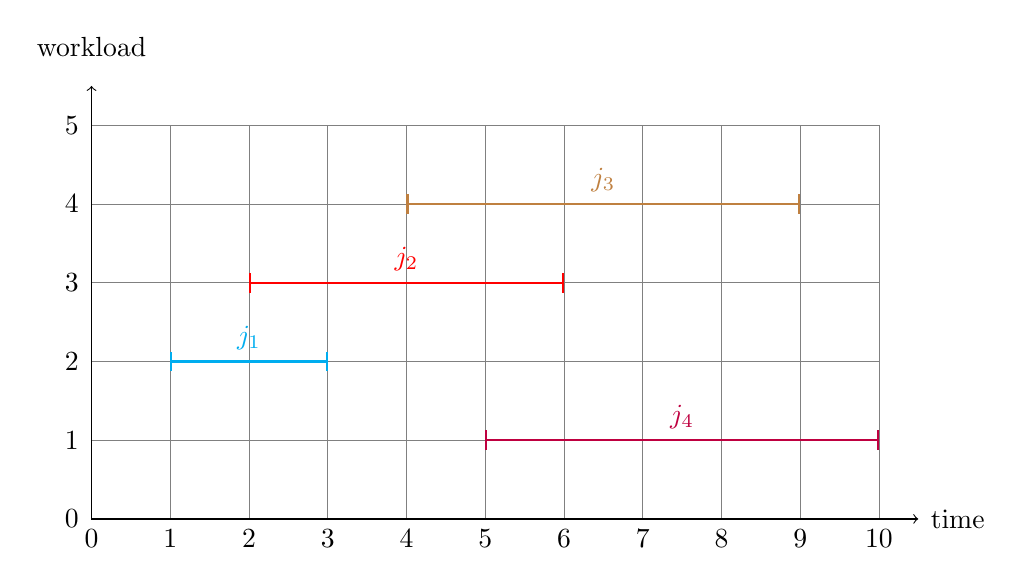
\begin{tikzpicture}
    \draw[help lines] (0,0) grid (10,5);
    \draw[<->] (0,5.5) -- (0,0) -- (10.5,0);
    \foreach \y in {0,1,...,5} \draw (-0.25,\y) node {\y};
    \foreach \x in {0,1,...,10} \draw (\x, -0.25) node {\x};
    \draw (11,0) node {time};
    \draw (0,6) node {workload};
    \draw[|-|,cyan,thick] (1,2) -- (3,2);
    \draw[cyan] (2,2.3) node {$j_1$};
    \draw[|-|,red,thick] (2,3) -- (6,3);
    \draw[red] (4,3.3) node {$j_2$};
    \draw[|-|,brown,thick] (4,4) -- (9,4);
    \draw[brown] (6.5,4.3) node {$j_3$};
    \draw[|-|,purple,thick] (5,1) -- (10,1);
    \draw[purple] (7.5,1.3) node {$j_4$};
  \end{tikzpicture}
\end{figure}

We introduce two parameters: $D$ and $S$ which will be the maximal
deadline and the maximal workload. So, for any job
$j_i=(a_i,s_i,d_i)$ we have $s_i\leq S$, $d_i\leq \Delta$.
The speeds that our processor can choose are represented by a finite
set $\V\subset\N$. To minimize the expected energy consumption, we
need to have some probability informations on the jobs that will
come, that will be explained later.

\subsection{The remaining work function}
First, a quick reminder of what a Markov Decision Process is. MDPs are
made to model decision making where the outcome depends on what action
you choose and randomness. For example, I am in location A, I want to
go to location B by taking a cab and I want to go there
\textbf{safely}. So I will choose the cab with the well maintened car
but my security will also depend on the sanity of the driver which
will be determined at random. In the end, I will either end up in
location B with probability $p_i$ or at the hospital with probability
$1-p_i$ with. Here, we did only one choice but in general, MDPs are
used to model longer periods of time.\\

\begin{figure}
  \centering
 \caption{A example of a MDP}
  \label{fig:mdp}
  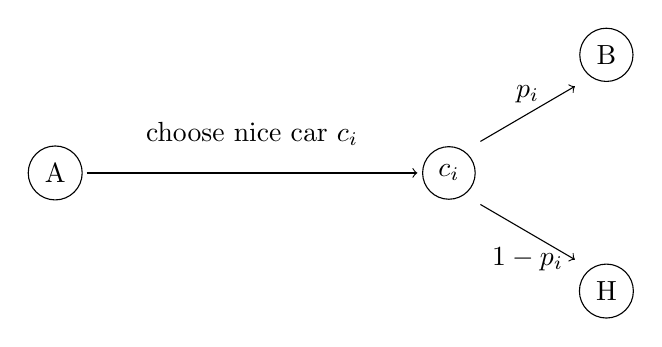
\begin{tikzpicture}
    \draw (0,0) node[circle,draw] {A};
    \draw[->] (0.4,0) -- (4.6,0);
    \draw (2.5,0.5) node {choose nice car $c_i$};
    \draw (5,0) node[circle,draw] {$c_i$};
    \draw (7,1.5) node[circle,draw] {B};
    \draw (7,-1.5) node[circle,draw] {H};
    \draw[->] (5.4,0.4) -- (6.6, 1.1);
    \draw (6,1) node {$p_i$};
    \draw (6,-1.1) node {$1-p_i$};    
    \draw[->] (5.4,-0.4) -- (6.6, -1.1);  
  \end{tikzpicture}
\end{figure}

On figure~\ref{fig:mdp}, from state A we can go to B or to H, so our state
space is \{A,B,H\}. In our problem, state space will be the space of
the remaining functions. To execute the jobs that the processor has
received, we are gonna use the strategy of ``Earliest Deadline
First'', so in priority we do the jobs that needs to be done the
sooner. From there, the only useful information is the workload that
has to be done over time (we do not care about scheduling). From there
we can introduce a function: $D(\cdot)$ where $D(t)$ is the amount of
work that must be done before time $t$. For example, on
figure~\ref{fig:D}, I have represented the function $D(\cdot)$ in
green for the list of jobs of the figure~\ref{fig:jobs}. We can also
define the function $A(\cdot)$ where $A(t)$ is the amount of work that
the processor has received at time $t$, it is represented in red on
figure~\ref{fig:D}.

\begin{figure}
  \centering
  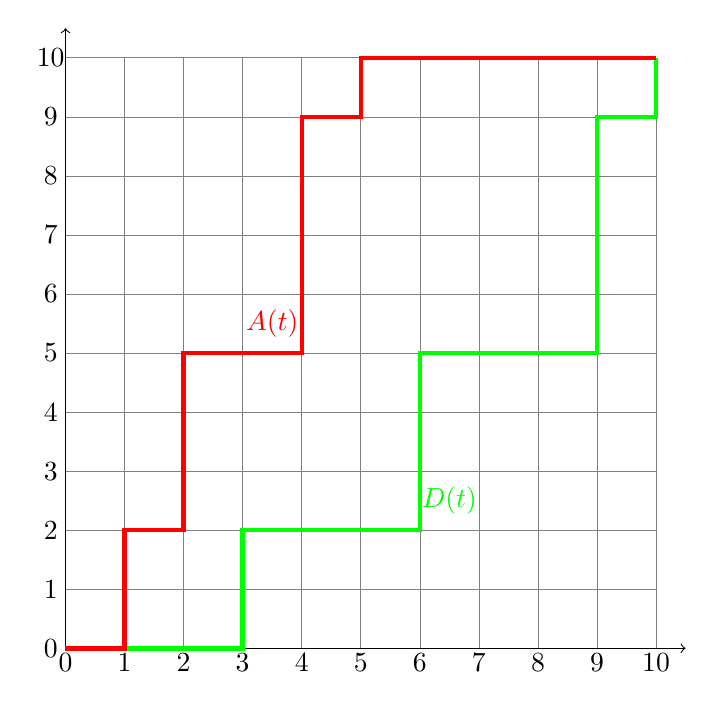
\begin{tikzpicture}[scale=0.75]
    \draw[help lines] (0,0) grid (10,10);
    \foreach \x in {0,1,...,10} \draw (\x,-0.25) node {\x};
    \foreach \y in {0,1,...,10} \draw (-0.25,\y) node {\y};
    \draw[<->] (0,10.5) -- (0,0) -- (10.5,0);
    \draw[green,ultra thick] (0,0) -- (3,0) -- (3,2) -- (6,2) -- (6,5)
    -- (9,5) -- (9,9) -- (10,9) -- (10,10);
    \draw[green] (6.5,2.5) node {$D(t)$};
    \draw[red, ultra thick] (0,0) -- (1,0) -- (1,2) -- (2,2) -- (2,5)
    -- (4,5) -- (4,9) -- (5,9) -- (5,10) -- (10,10);
    \draw[red] (3.5,5.5) node {$A(t)$};
  \end{tikzpicture}
  \caption{Function $D(\cdot)$ and $A(\cdot)$}
  \label{fig:D}
\end{figure}

The remaining work at time $t$ is a step increasing function
$w_t(\cdot)$ and $w_t(u)$ is the workload that needs to be done before
$t+u$. Because all jobs have a deadline $\Delta$, all $w_t$ are
defined on $\llbracket 0,\Delta\rrbracket$. For example, on figure
\ref{fig:jobs}, suppose we are at $t=2$ and that our processor has not
worked yet. We can see on the graph that $j_1$ and $j_2$ are known by
the processor because $a_1,a_2\leq 2$. We can see the remaining work
function on figure~\ref{fig:workfun}. The first step represents the
workload of $j_1$ that has to be finished before $t=3$. The second
step represents the workload of $j_2$ that has to be finished before
$t=6$. 

\begin{figure}
  \centering
  \caption{Remaining work function $w_2(\cdot)$.
    Keep in mind that for $w_t(\cdot)$, $w_t(u)$ represents the
  remaining work that has to be done at time $t+u$.}
  \label{fig:workfun}
  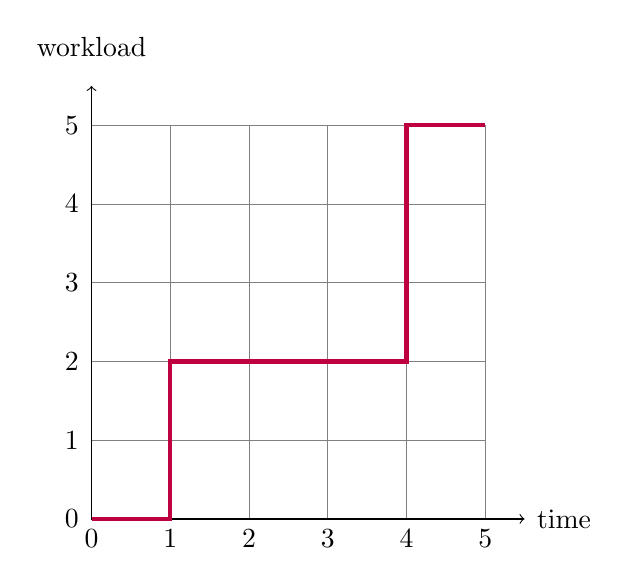
\begin{tikzpicture}
    \draw[help lines] (0,0) grid (5,5);
    \draw[<->] (0,5.5) -- (0,0) -- (5.5,0);
    \draw (6,0) node {time};
    \draw (0,6) node {workload};
    \foreach \x in {0,1,...,5} \draw (\x, -0.25) node {\x};
    \foreach \y in {0,1,...,5} \draw (-0.25,\y) node {\y};
    \draw[purple,ultra thick] (0,0) -- (1,0) -- (1,2) -- (4,2) -- (4,5)
    -- (5,5);
  \end{tikzpicture}
\end{figure}



I will call the space of the remaining work functions $\W$. From state
$w$, which state $w'\in\W$ can we obtain ? To know that, we need some
definitions.

\begin{defi}
  $\T$ is the shift operator defined as:
  \[ \forall x\in\R,\T f(x) = f(x+1)\]
\end{defi}

\begin{defi}
  $H_t$ is the heavyside function defined as:
  \[ H_t(x) =
    \begin{cases}
      0 & x<t \\
      1 & x\geq t
    \end{cases}
  \]
\end{defi}

\begin{defi}
  $f^+$ is the positive part of function $f$ defined as:
  \[
    \forall x\in\R, f^+(x)=\max(0,f(x))
  \]
\end{defi}

Now, suppose a job $j=(a,s,d)$ arrives at time $t=a$. If the processor
speed at time $t-1$ is $v_{t-1}$ then we have:
\begin{equation}
  \label{eq:nextw}
  w_t(\cdot)=\T[(w_{t-1}(\cdot)-v_{t-1})^+]+s\times H_d(\cdot)
\end{equation}


\end{document}